%! suppress = EscapeAmpersand
%! suppress = EscapeUnderscore
The earliest known forms of probability and statistics were developed by Arab mathematicians studying cryptography 
between the 8th and 13th centuries. The modern mathematical theory of probability has its roots in attempts to 
analyse games of chance. \v

Initially, probability theory mainly considered discrete events, and its methods were mainly combinatorial.
Eventually, analytical considerations compelled the incorporation of continuous variables into the theory. This
culminated in modern probability theory, on foundations laid by Andrey Nikolaevich Kolmogorov. Kolmogorov combined
the notion of sample space and measure theory and presented his axiom system for probability theory in 1933. This
became the mostly undisputed axiomatic basis for modern probability theory. We will follow a similar path, first by
defining the notion of sample space and measure theory and then by combining them in order to develop probability
theory.

\section{Sample Space}

\bd[Random Experiment]
A \textbf{random experiment} is an experiment, trial, or observation with the following properties:
\bit
\item It can be repeated numerous times under the same conditions.
\item The experiment can have more than one outcome.
\item Each possible outcome can be specified in advance.
\item The outcome of the experiment depends on chance.
\eit
\ed

\bd[Outcome]
An \textbf{outcome} is a possible result of a random experiment or trial. Each possible outcome of a particular 
experiment is unique, and different outcomes are mutually exclusive (only one outcome will occur on each trial of the
experiment). 
\ed

Given a random experiment and its possible outcomes, we can define the concept of a sample space and an event as 
follows.

\bd[Sample Space]
\textbf{Sample space} $S$ of a random experiment or random trial is the set of all possible outcomes or results of that 
experiment.
\ed

\bd[Event]
An \textbf{event} $A$ is a subset of the sample space.
\ed

\fig{event}{0.3}

Now that we have attached a set representation to events, we can use the usual set theory to define basic operations 
on events.

\bd[Complement Event]
The \textbf{complement} of an event $A$ denoted by $A^{C}$ is the set of elements not in A, within the sample space $S$:
\bse
A^{C} = \{x:x\in S \mid x \notin A \}
\ese
\ed

\vspace{-5pt}

\fig{complement}{0.1}

\bd[Union]
The \textbf{union} of two events A and B is the event containing elements which are in A, in B, or in both A and B\@.
\bse
A\cup B=\{x:x\in A{\text{ or }}x\in B\}
\ese
\ed

\fig{union}{0.2}

\bd[Intersection]
The \textbf{intersection} of two events A and B, is the event containing all elements of A that also belong to B (or 
equivalently, all elements of B that also belong to A).
\bse
A\cap B=\{x:x\in A{\text{ and }}x\in B\}
\ese
\ed

\vspace{-5pt}

\fig{intersection}{0.2}

\bd[Mutually Exclusive Events]
Two events A and B are called \textbf{mutually exclusive} if the intersection of the events is equal to the empty set.
\bse
A\cap B= \emptyset
\ese
\ed

\fig{mutually_exclusive}{0.7}

Based on the set nature of events we can give a first naive definition of probability as follows.

\bd[Naive Probability]
\textbf{Naive probability} of an event $A$ is defined as the fraction of favorable outcomes over all possible outcomes.
\bse
P(A) = \frac{\text{number of favorable outcomes}}{\text{number of total outcomes}}
\ese
\ed

\v

The naive definition of probability assumes that all favourable events are equally likely to be picked and that we 
are dealing with a finite sample space. Both assumptions of this definition add some limitations to the theory, hence
we need to give a more formal and mathematical definition of probability. In order to do show we first need to review
one of the fundamental concepts in mathematics called ``measure theory''. \v

To sum up, what we really want to do is to attach a number (measure) to every event (subset) of sample space (set) 
that we will eventually interpret as probability. Since a sample space, and an event are just sets, for now we can 
forget everything related to probability, and treat them like plain sets. Hence, what we are trying to do is to
assign a number to every subset of a set. This is exactly what measure theory deals with!

\section{Measure Theory}

A measure on a set is a systematic way to assign a number to each suitable subset of that set, intuitively 
interpreted as its size. In this sense, a measure is a generalization of the concepts of length, area, and volume. 
A particularly important example is the Lebesgue measure on a Euclidean space, which assigns the conventional 
length, area, and volume of Euclidean geometry to suitable subsets of the Euclidean space. Subsequently, measure 
theory was developed in successive stages during the late 19th and early 20th centuries. The main application of 
measure theory is in the foundations of the Lebesgue integral, in Kolmogorov's axiomatisation of probability theory 
that we will see right after. \v

Technically, a measure is a function that assigns a non-negative real number to (certain) subsets of a set $X$. It
must further be countably additive: the measure of a large subset that can be decomposed into a finite (or countably
infinite) number of smaller disjoint subsets is equal to the sum of the measures of the smaller subsets. In general,
if one wants to associate a consistent size to each subset of a given set while satisfying the other axioms of a
measure, one only finds trivial examples like the counting measure. This problem was resolved by defining measure
only on a sub-collection of all subsets, the so-called ``measurable subsets'', which are required to form a
``$\sigma$-algebra''. This means that countable unions, countable intersections and complements of measurable subsets
are measurable. Non-measurable sets in a Euclidean space, on which the Lebesgue measure cannot be defined
consistently, are necessarily complicated in the sense of being badly mixed up with their complement. Indeed, their
existence is a non-trivial consequence of the axiom of choice.

\subsection{Basic Definitions}

\bd[$\sigma$-algebra] Let $M$ be a non-empty set. A collection $\Sigma\subseteq\mathscr{P}(M)$ of subsets of $M$ is
called a \textbf{$\sigma$-algebra} for $M$ if it includes $M$ itself, it is closed under complement, and it is closed
under countable unions:
\ben[label=(\roman*)]
\item $M\in \Sigma$.
\item If $A\in \Sigma$, then $M\setminus A \in \Sigma$.
\item For any sequence $\{A_n\}_{n\in \N}$ in $\Sigma$ we have $\bigcup_{n=0}^{\infty}A_n\in\Sigma$.
\een
\ed

\be
For example if $\Sigma = \{a, b, c, d\}$ is a sample space, one possible $\sigma$-algebra on sample space $\Sigma$ is
$\mathcal{F} = \{\emptyset, \{a, b\}, \{c, d\}, \{a, b, c, d\} \}$, where $\emptyset$ is the empty set.
\ee

If we relax the third condition so that it applies only to finite (rather than countable) unions, we obtain the
notion of an \emph{algebra}, often called an \emph{algebra of sets} in order to distinguish it from the notion of
algebra as a vector space equipped with a bilinear product, with which it has nothing to do. Note that by condition
(ii) and De Morgan's laws, condition (iii) can be equivalently stated in terms of intersections rather than unions.
Recall that De Morgan's laws ``interchange'' unions with intersections and vice-versa under the complement operation.
That is, if $M$ is a set and $\{A_i\}_{i\in I}$ is a collection of sets, then:
\bse
M \setminus \biggl(\bigcup_{\,i\in I}A_i\biggr) = \bigcap_{i\in I} (M\setminus A_i \quad \text{and} \quad
M \setminus \biggl(\bigcap_{\,i\in I}A_i\biggr) = \bigcup_{i\in I} (M\setminus A_i)
\ese

\bt[]
Let $M$ be a set and let $\Sigma$ be a $\s$-algebra on $M$. Let $\{ A_n \}_{n\in \N}$ be a sequence in $\Sigma$.
Then, for all $k\in \N$, we have:
\ben[label=(\roman*)]
\item $\bigcup_{n=0}^k{A_n} \in \Sigma$.
\item $\bigcap_{n=0}^{\infty}{A_n} \in \Sigma \ $ and $\ \bigcap_{n=0}^k{A_n} \in \Sigma$.
\een
\et

\bq
\ben[label=(\roman*)]
\item Let the sequence $\{B_n\}_{n\in \N}$ be defined as follows:
\bse
B_n = \begin{cases} A_n \quad &\t{if }\ 0 \leq n \leq k\\ \varnothing \quad &\t{if }\ n > k \end{cases}
\ese

Then, $\{B_n\}_{n\in \N}$ is a sequence in $\Sigma$, so $ \bigcup_{n=0}^{\infty}{B_n} \in \Sigma$. Hence, we have:
\bse
\bigcup_{n=0}^{\infty}{B_n} = \biggl(\bigcup_{\,n=0}^{k}{B_n}\biggr) \cup
\biggl(\bigcup_{\, n=k+1}^{\infty}{\negmedspace B_n}\biggr)=\bigcup_{n=0}^k{A_n}
\ese

and thus $\bigcup_{n=0}^k{A_n} \in \Sigma$.
\item As $\{A_n\}_{n\in \N}$ is a sequence in $\Sigma$, so is $\{M\setminus A_n\}_{n\in \N}$ and hence
$\bigcup_{n=0}^{\infty}{(M\setminus A_n)} \in \Sigma$. Thus, we also have:
\bse
M \setminus \biggl( \bigcup_{\,n=0}^{\infty}{(M\setminus A_n)} \biggr) \in \Sigma
\ese

and since $M\setminus(M\setminus A_n)=A_n$, by De Morgan's laws, $\bigcap_{n=0}^{\infty}{A_n} \in \Sigma$. That this
holds for finite intersections is shown by defining $\{B_n\}_{n\in \N}$ as above. \qedhere
\een
\eq

A $\sigma$-algebra is closed under countably infinite unions (by definition) but also under countably infinite
intersections and finite unions and intersections. \v

\bd [Measurable Space / Borel Space]
A \textbf{measurable space} (or \textbf{Borel space}) is a pair $(M,\Sigma)$ where $M$ is a set and $\Sigma$ is a
$\sigma$-algebra on $M$.
\ed

\bd [Measurable Subsets]
The elements of $\Sigma$ of a measurable space $(M,\Sigma)$ are called \textbf{measurable subsets} of $M$.
\ed

Our goal in this chapter is to assign volumes (i.e.\ measures) to subsets of a given set. Of course, we would also
like this assignment to satisfy some sensible conditions. However, it turns out that one cannot sensibly assign
volumes to any arbitrary collection of subsets of a given set. It is necessary that the collection of subsets be a
$\sigma$-algebra. In addition, just like in topology openness and closeness are not properties of subsets but
properties of subsets with respect to a choice of topology, so does measurability of subsets only make sense with
respect to a choice of $\sigma$-algebra. In particular, a given subset could be measurable with respect to some
$\sigma$-algebra and not measurable with respect to some other $\sigma$-algebra.

\be
The pair $(M,\mathscr{P}(M))$ is a measurable space for any set $M$. Of course, just like the discrete topology is
not a very useful topology, the power set $\mathscr{P}(M)$ is not a very useful $\sigma$-algebra on $M$, unless $M$
is countable.
\ee

\bd [Measure]
Let $(M,\Sigma)$ be a measurable space. A \textbf{measure} on $(M,\Sigma)$ is a function:
\bse
\mu\cl\Sigma\to[0,\infty]
\ese

where $[0,\infty] \coloneqq \{r\in\overline{\R}\mid r \geq 0\}$, such that:
\ben[label=(\roman*)]
\item $\mu(\varnothing)=0$.
\item For any pairwise disjoint sequence $\{A_n\}_{n\in \N}$ in $\Sigma$ (i.e.\ with $A_i\cap A_j = \varnothing \forall
i\neq j$), we have:
\bse
\mu\biggl(\bigcup_{\,n=0}^{\infty}A_n\biggr) = \sum_{n=0}^{\infty}\mu(A_n)
\ese

where $\overline{\R}$ is the so called ``extended real line'' with $\overline{\R} \coloneqq \R \cup \{-\infty,
+\infty\}$, where the symbols $-\infty$ and $+\infty$ (the latter often denoted simply by $\infty$) satisfy:
\bse
\forall \, r \in \overline{\R} : \ -\infty\leq r \leq \infty
\ese

with strict inequalities if $r\in\R$.
\een
\ed

Both sides of the equation in part (ii) of the definition of measure might take the value $\infty$. There are two
possible reasons why $\sum_{n=0}^{\infty}\mu(A_n)$ might be infinite. It could be that $\mu(A_n) = \infty$ for some
$n\in \N$ or, alternatively, it could be that $\mu(A_n) < \infty$ for all $n \in \N$ but the sequence of partial sums
$\{ \sum_{i=0}^{n}\mu(A_i)\}_{n\in\N}$, which is an increasing sequence since $\mu$ is non-negative by definition, is
not bounded above. \v

\bd [Measure Space]
A \textbf{measure space} is a triple $(M,\Sigma,\mu)$ where $(M,\Sigma)$ is a measurable space and
$\mu\cl\Sigma\to[0,\infty]$ is a measure on $M$.
\ed

\be \
Let $M=\N$ and $\Sigma=\mathscr{P}(\N)$. Define $\mu : \Sigma \to [0, \infty]$ by:
\bse
\mu(A) = |A| \coloneqq
\begin{cases}
n & \text{ if $A$ is a finite set with $n$ elements}\\ \infty & \text{ if $A$ is not a finite set}
\end{cases}
\ese

Then, by definition, $\mu(\vn) =0$. Moreover, if $\{A_n\}_{n\in\N}$ is a pairwise disjoint sequence in $\Sigma$ such
that all but a finite number of $A_n$'s are empty and each $A_n$ has a finite number of elements, we have:
\bse
\mu \biggl( \bigcup_{\,n=0}^{\infty}A_n\biggr) = \sum_{n=0}^{\infty}\mu(A_n)
\ese

by counting elements. Otherwise, that is, if an infinite number of $A_n$'s are non-empty or if at least one $A_n$ is
infinite, then:
\bse
\mu \biggl( \bigcup_{\,n=0}^{\infty}A_n\biggr) = \infty = \sum_{n=0}^{\infty}\mu(A_n)
\ese

\v

and thus, the triple $(\N,\mathscr{P}(\N),\mu)$ is a measure space. The measure $\mu$ on $(\N,\mathscr{P}(\N))$ is
called ``counting measure'', and it is the usual measure on countable measurable spaces.
\ee

Now let's give some basic definitions involving measures and measure spaces.

\bd [Finite Measure]
Let $(M,\Sigma,\mu)$ be a measure space. The measure $\mu$ is said to be \textbf{finite} if there exists a sequence
$\{A_n\}_{n\in\N}$ in $\Sigma$ such that $\bigcup_{n=0}^{\infty}A_n=M$ and:
\bse
\forall \, n \in \N : \ \mu(A_n)<\infty
\ese
\ed

\be
The counting measure on $(\N,\mathscr{P}(\N))$ is finite. To see this, define $A_n \coloneqq \{n\}$. Then, clearly
$\bigcup_{n=0}^{\infty}A_n=\N$ and $\mu(A_n)=|\{n\}|=1<\infty$ for all $n\in \N$.
\ee

What follows is two definitions that are not really about measures and measure spaces, but we need them in order to
define the notion of ``complete measure''.

\bd [Null Set / Set Of Measure Zero]
Let $(M,\Sigma,\mu)$ be a measure space. If $A\in\Sigma$ is such that $\mu (A)=0$, then $A$ is called a \textbf{null
set} or a \textbf{set of measure zero}.
\ed

\bd [Almost Everywhere]
Let $(M,\Sigma,\mu)$ be a measure space and let $P$ be some property or statement. We say that $P$ holds
\textbf{almost everywhere} on $M$ if:
\bse
\exists \, Z\in \Sigma : \ \mu(Z) = 0 \, \text{ and } \, \forall \, m\in M\setminus Z : \, P(m)
\ese
\ed

In other words, the property $P$ is said to hold almost everywhere on $M$ if it holds everywhere on $M$ except for a
null subset of $M$.

\bd [Complete Measure]
A measure $\mu\cl \Sigma\to [0,\infty]$ is said to be \textbf{complete} if every subset of every null set is
measurable, i.e.\ :
\bse
\forall \, A\in \Sigma :\forall \, B\in\mathscr{P}(A) : \ \mu(A)=0 \, \Rightarrow \, B\in\Sigma
\ese
\ed

Note that since for any $A,B\in\Sigma$, $B\subseteq A$ implies $\mu(B) \leq\mu(A)$, it follows that every subset of a
null set, if measurable, must also be a null set.

\bd [Translation-Invariant Measure]
Let $(M,\Sigma,\mu)$ be a measure space and let $(M,+,\cdot)$ be a vector space. The measure $\mu$ is said to be
\textbf{translation-invariant} if:
\bse
\forall \, m\in M : \forall \, A\in \Sigma : \quad A+m\in\Sigma\ \text{and}\ \mu(A+m)=\mu(A)
\ese

where $A+m \coloneqq \{a+m\mid a\in A\}$.
\ed

Finally, let's see and prove some properties of the measure.

\bt[]
Let $(M,\Sigma,\mu)$ be a measure space.
\ben[label=(\roman*)]
\item If $A_0,\ldots,A_k \in \Sigma$ and $A_i \cap A_j = \varnothing$ for all $0\leq i\neq j\leq k$, then:
\bse
\mu \biggl( \bigcup_{\,n=0}^{k}A_n\biggr) = \sum_{n=0}^{k}\mu(A_n)
\ese

\item If $A,B\in \Sigma$ and $A \subseteq B$, then $\mu(A) \leq \mu(B)$.
\item If $A,B \in \Sigma$, $A \subseteq B$ and $\mu(A)<\infty$, then $ \mu (B\setminus A)=\mu(B)-\mu(A)$.
\item Continuity from below: Let $\{A_n\}_{n\in \N}$ be a sequence in $\Sigma$. If $\{A_n\}_{n\in \N}$ is increasing,
i.e.\ $A_n\subseteq A_{n+1}$ for all $n \in \N$, then:
\bse
\mu \biggl( \bigcup_{\,n=0}^{\infty}A_n\biggr) = \lim_{n \to \infty} \mu(A_n)
\ese

\item Continuity from above: Let $\{A_n\}_{n\in \N}$ be a sequence in $\Sigma$. If $\mu(A_0)<\infty$ and
$\{A_n\}_{n\in \N}$ is decreasing, i.e.\ $ A_{n+1}\subseteq A_n$ for all $n \in \N$, then:
\bse
\mu \biggl( \bigcap_{\,n=0}^{\infty}E_n\biggr) = \lim_{n \to \infty} \mu(A_n)
\ese

\item The measure $\mu$ is countably sub-additive. That is, for any sequence $\{A_n\}_{n\in\N}$ in $\Sigma$, we have:
\bse
\mu\biggl(\bigcup_{\,n=0}^{\infty}A_n\biggr)\leq \sum_{n=0}^{\infty}\mu(A_n)
\ese
\een
\et

As an exercise let's prove these statements.

\ben[label=(\roman*)]
\item Let $A_n=\varnothing$ for all $n>k$. Then, $\{A_n\}_{n\in\N}$ is a pairwise disjoint sequence in $\Sigma$ and
hence, we have:
\bse
\mu \biggl( \bigcup_{\,n=0}^{k}A_n\biggr) =\mu \biggl( \bigcup_{\, n=0}^{\infty}A_n\biggr)
= \sum_{n=0}^{\infty}\mu (A_n)= \sum_{n=0}^{k}\mu(A_n)
\ese

\item We have $B=A\cup (B\setminus A)$ and $A\cap (B\setminus A) =\varnothing$. Hence, by part (i):
\bse
\mu(B)= \mu(A\cup (B\setminus A))=\mu(A)+\mu ( B\setminus A)
\ese

and since $\mu ( B\setminus A)\geq 0$, we have $ \mu(A) \leq \mu(B)$.

\item By decomposing $B$ as above and rearranging, we immediately get:
\bse
\mu(B\setminus A)=\mu(B)-\mu(A)
\ese

Note, however, that this only makes sense if $\mu(A)<\infty$, for otherwise we must also have $\mu(B)=\infty$ by part
(ii), and then $\mu(B)-\mu(A)$ would not be defined.
\item Define $B_0 \coloneqq A_0$ and $B_n \coloneqq A_n\setminus A_{n-1}$. Then, $\{ B_n \}_{n\in\N}$ is a pairwise
disjoint sequence in $\Sigma$ such that:
\bse
\bigcup_{i=0}^n B_i = A_n\qquad \text{ and }\qquad \bigcup_{n=0}^{\infty} A_n=\bigcup_{n=0}^{\infty} B_n
\ese

Hence:
\bse
\mu \biggl(\bigcup_{\,n=0}^{\infty}A_n\biggr) = \mu \biggl(\bigcup_{\, n=0}^{\infty}B_n\biggr)
= \sum_{n=0}^{\infty}\mu(B_n) = \lim_{n \to \infty}\sum_{i=0}^n \mu(B_i)
= \lim_{n \to \infty}\mu \biggl(\bigcup_{\, i=0}^{n}B_n\biggr) = \lim_{n \to \infty} \mu(A_n)
\ese

\item Define $B_n \coloneqq A_0\setminus A_n$. Then, $B_n \subseteq B_{n+1}$ for all $n \in \N$ and thus, by part (i),
we have:

\bse
\mu \biggl( \bigcup_{\,n=0}^{\infty}B_n\biggr) = \lim_{n \to \infty} \mu (B_n)
= \lim_{n \to \infty} ( \mu(A_0)-\mu (A_n)) = \mu(A_0)-\lim_{n \to \infty} \mu(A_n)
\ese

Note that, by definition of $B_n$, we have:
\bse
\bigcup_{n=0}^{\infty}B_n = A_0 \setminus \bigcap_{\,n=0}^{\infty}A_n.
\ese

Since $\mu(A_0)<\infty$, it follows from the previous proposition that:
\bse
\mu(A_0)-\mu \biggl(\bigcap_{\,n=0}^{\infty}A_n\biggr) = \mu \biggl( A_0 \setminus \bigcap_{n=0}^{\infty}A_n\biggr)
= \mu \biggl(\bigcup_{\,n=0}^{\infty}B_n\biggr) = \mu(A_0)-\lim_{n \to \infty} \mu(A_n)
\ese

Therefore, we have:
\bse
\mu \biggl( \bigcap_{n=1}^{\infty}A_n\biggr) = \lim_{n \to \infty} \mu(A_n)
\ese

\item We will prove this in steps.
\ben
\item First, we show that $\mu(A\cup B)\leq \mu(A)+\mu(B)$ for any $A, B\in\Sigma$. Note that, for any pair of sets
$A$ and $B$, the sets $A\setminus B$, $B\setminus A$ and $A\cap B$ are pairwise disjoint and their union is $A\cup B$. \v

\begin{center}
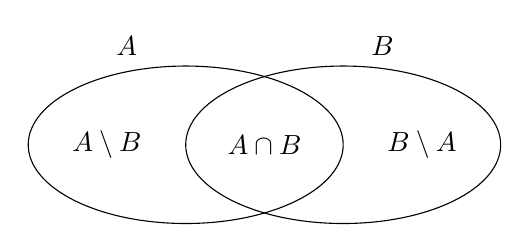
\begin{tikzpicture}[scale=0.5]
\draw (-3.5,1.5) ellipse (4 and 2);
\draw (0.5,1.5) ellipse (4 and 2);
\node at (-5.5,1.5) {$A\setminus B$};
\node at (-1.5,1.5) {$A\cap B$};
\node at (2.5,1.5) {$B\setminus A$};
\node at (-5,4) {$A$};
\node at (1.5,4) {$B$};
\end{tikzpicture}
\end{center}

By writing $A = (A\setminus B ) \cup (A\cap B)$ and $B = (B\setminus A ) \cup (A\cap B)$ and using the additivity and
positivity of $\mu$, we have:
\bi{rCl}
\mu(A)+\mu(B)& = &\mu((A\setminus B ) \cup (A\cap B))+\mu((B\setminus A ) \cup (A\cap B))\\
& = &\mu(A\setminus B ) + 2\mu(A\cap B)+\mu(B\setminus A )\\
& = &\mu(A\cup B ) + \mu(A\cap B)\\
& \geq & \mu(A\cup B )
\ei

\item We now extend this to finite unions by induction. Let $\{A_n\}_{n\in\N}$ be a sequence in $\Sigma$ and suppose
that:
\bse
\mu\biggl(\bigcup_{\,i=0}^{n}A_i\biggr)\leq \sum_{i=0}^{n}\mu(A_i)
\ese

\v

for some $n\in \N$. Then, by part (a), we have:
\bse
\mu\biggl(\bigcup_{\,i=0}^{\,n+1}A_i\biggr) = \mu\biggl (A_{n+1}\cup\bigcup_{i=0}^{n}A_i\biggr) \leq \mu (A_{n+1})
+\mu\biggl(\bigcup_{\,i=0}^{n}A_i\biggr) \leq \mu (A_{n+1}) +\sum_{i=0}^{n}\mu(A_i) = \sum_{i=0}^{n+1}\mu(A_i)
\ese

Hence, by induction on $n$ with base case $n=1$ and noting that the case $n=0$ is trivial (it reduces to $\mu(A_0)
=\mu(A_0)$), we have:
\bse
\forall \, n \in \N : \ \mu\biggl(\bigcup_{\,i=0}^{n}A_i\biggr)\leq \sum_{i=0}^{n}\mu(A_i)
\ese

\item Let $\{A_n\}_{n\in\N}$ be a sequence in $\Sigma$. Define $B_n \coloneqq \bigcup_{i=0}^n A_n$. Then,
$\{B_n\}_{n\in\N}$ is an increasing sequence in $\Sigma$. Hence, by continuity from above of $\mu$, we have:
\bse
\mu\biggl(\bigcup_{\,n=0}^{\infty}A_n\biggr) = \mu\biggl(\bigcup_{\, n=0}^{\infty}B_n\biggr) = \lim_{n\to\infty}\mu
(B_n) = \lim_{n\to\infty}\mu\biggl(\bigcup_{\,i=0}^{n}A_i\biggr) \leq \lim_{n\to\infty}\sum_{i=0}^n\mu(A_i)
= \sum_{i=0}^\infty\mu(A_i)
\ese

which is what we wanted. \qedhere
\een
\een

\subsection{Borel $\sigma$-algebras}

We have already remarked the parallel between topologies and $\sigma$-algebras. A further similarity stems from the
fact that, just like for topologies, interesting $\sigma$-algebras are hardly ever given explicitly, except in some
simple cases. In general, they are defined implicitly by some membership condition.

\bt[]
Let $M$ be a set and let $\{ \Sigma_i : i \in I\}$ be a collection of $\s$-algebras on $M$. Define the set:
\bse
\Sigma \coloneqq \bigcap_{i\in I}\Sigma_i = \{ A \in \mathscr{P}(M) \mid A \in \Sigma_i, \forall \, i \in I \}
\ese

Then, $\Sigma$ is a $\s$-algebra on $M$.
\et

\bq
We simply check that $\Sigma$ satisfies the defining properties of a $\sigma$-algebra:
\ben[label=(\roman*)]
\item We have $M \in \Sigma_i$ for all $i \in I$ and hence, $ M \in \Sigma$.
\item Let $A \in \Sigma$. Then, $A \in \Sigma_i$ for all $i \in I$ and, since each $\Sigma_i$ is a $\s$-algebra, we
also have $M\setminus A \in \Sigma_i$ for all $i\in I$. Hence, $M\setminus A \in \Sigma$.
\item Let $\{A_n\}_{n\in\N}$ be a sequence in $\Sigma$. Then, $\{A_n\}_{n\in\N}$ is a sequence in each $\Sigma_i$. Thus:
\bse
\forall \, i\in I : \ \bigcup_{n=0}^{\infty}{A_n} \in \Sigma_i
\ese

Hence, we also have $\bigcup_{n=0}^{\infty}{A_n} \in \Sigma$. \qedhere
\een
\eq

\bd [Generating Set]
Let $M$ be a set and let $\mathcal{E}\subseteq\mathscr{P}(M)$ be a collection of subsets of $M$. The $\sigma$-algebra
\emph{generated} by $\mathcal{E}$, denoted $\sigma(\mathcal{E})$, is the smallest $\sigma$-algebra on $M$ containing
all the sets in $\mathcal{E}$. That is:
\bse
A\in\sigma(\mathcal{E}) \quad \Leftrightarrow \quad \text{for all $\sigma$-algebras }\Sigma
\text{ on } M :\ \mathcal{E}\subseteq \Sigma \, \Rightarrow\, A\in \Sigma
\ese

or, by letting $\{\Sigma_i\mid i\in I\}$ be the collection of $\sigma$-algebras on $M$ such that
$\mathcal{E}\subseteq \Sigma$:
\bse
\sigma(\mathcal{E}) \coloneqq \bigcap_{i\in I}\Sigma_i
\ese

The set $\mathcal{E}$ is called a \textbf{generating set} for $\sigma (\mathcal{E})$.
\ed

Observe that the second characterisation makes it manifest that $\sigma (\mathcal{E})$ is indeed a $\sigma$-algebra
on $M$ by the previous proposition.

\bt[]
Let $(M,\Sigma)$ be a measurable space. Then, $\Sigma=\sigma(\mathcal{E})$ for some $\mathcal{E}\subseteq\mathscr{P}
(M)$. That is, every $\sigma$-algebra on $M$ is generated by some collection of subsets of $M$.
\et

This generating construction immediately allows us to link the notions of topology and $\sigma$-algebra on a set $M$
via the following definition.

\bd [Borel $\sigma$-algebra]
Let $(M,\mathcal{O})$ be a topological space. The \textbf{Borel $\sigma$-algebra} on $(M,\mathcal{O})$ is
$\sigma(\mathcal{O})$.
\ed

Recall that a topology on $M$ is a collection $\mathcal{O}\subseteq\mathscr{P}(M)$ of subsets of $M$ which contains
$\varnothing$ and $M$ and is closed under finite intersections and arbitrary (even uncountable) unions. The elements
of the topology are called \emph{open sets}. Of course, while there many choices of $\sigma$-algebra on $M$, if we
already have a topology $\mathcal{O}$ on $M$, then the associated Borel $\sigma$-algebra is very convenient choice of
$\sigma$-algebra since, as we will soon see, it induces a measurable structure which is compatible with the already
given topological structure. \v

This is, in fact, the usual philosophy in mathematics: we always let the stronger structures induce the weaker ones,
unless otherwise specified. For instance, once we have chosen an inner product on a space, we take the norm to be the
induced norm, which induces a metric, which in turn induces a topology on that space, from which we now know how to
obtain a canonical $\sigma$-algebra. \v

We remark that, while the Borel $\sigma$-algebra on a topological space is generated by the open sets, in general, it
contains much more that just the open sets.

\be
Recall that the standard topology on $\R$, denoted $\mathcal{O}_{\R}$, is defined by:
\bse
A\in \mathcal{O}_{\R} \quad \Leftrightarrow \quad \forall \, a\in A : \exists \, \varepsilon > 0 : \forall \, r \in
\R : \ |r-a|<\varepsilon \, \Rightarrow\, r\in A
\ese

In fact, the elements of $\mathcal{O}_{\R}$ are at most countable unions of open intervals in $\R$. Consider now the
Borel $\sigma$-algebra on $(\R,\mathcal{O}_{\R})$. Let $a<b$. Then, for any $n\in \N$, the interval $(a-\tfrac{1}{n},
b)$ is open. Hence, $\{(a-\tfrac{1}{n},b)\}_{n\in \N}$ is a sequence in $\sigma(\mathcal{O}_{\R})$. Since
$\sigma$-algebras are closed under countable intersections, we have:
\bse
\bigcap_{n=0}^{\infty}(a-\tfrac{1}{n},b) = [a,b) \in \sigma(\mathcal{O}_{\R})
\ese

Hence, $\sigma(\mathcal{O}_{\R})$ contains, in addition to all open intervals, also all half-open intervals. It is
not difficult to show that it contains all closed intervals as well. In particular, since singletons are closed,
$\sigma(\mathcal{O}_{\R})$ also contains all countable subsets of $\R$. In fact, it is non-trivial to produce a
subset of $\R$ which is not contained in $\sigma(\mathcal{O}_{\R})$.
\ee

\subsection{Lebesgue Measure (On $\R^d$)}

\bt[]
Let $\mathcal{O}_{\R^d}$ be the standard topology on $\R^d$. There exists a unique complete, translation-invariant
measure:
\bse
\lambda^d\cl\sigma(\mathcal{O}_{\R^d})\to[0,\infty]
\ese

such that for all $a_i,b_i\in\R$ with $1\leq i\leq d$ and $a_i<b_i$, we have:
\bse
\lambda^d\bigl([a_1,b_1)\times\cdots\times[a_d,b_d)\bigr) = \prod_{i=1}^d(b_i-a_i)
\ese
\et

\bd [Lebesgue Measure]
The measure $\lambda^d$ is called the \textbf{Lebesgue measure} on $\R^d$.
\ed

The superscript $d$ in $\lambda^d$ may be suppressed if there is no risk of confusion. Note that the Lebesgue measure
on $\R$, $\R^2$ and $\R^3$ coincides with the standard notions of length, area and volume, with the further insight
that these are only defined for the elements of the respective Borel $\sigma$-algebras.

\bt[]
The Lebesgue measure on $\R$ is finite.
\et

\bq
Consider the sequence $\{[a_n,a_n+1)\}_{n\in\N}$ where:
\bse
a_n = \begin{cases} -\tfrac{1}{2}n & \text{ if $n$ is even}\\ \tfrac{1}{2}(n+1) & \text{ if $n$ is odd}. \end{cases}
\ese

\v

That is, $\{a_n\}_{n\in\N}$ is the sequence $(0,1,-1,2,-2,3,-3,\ldots)$.

\vspace{15pt}

\begin{center}
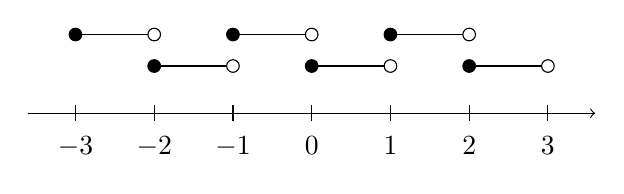
\begin{tikzpicture}
\foreach \i in {-3,-2,-1,0,1,2,3} {
\draw (\i,0.1)--(\i,-0.1) node[below=2pt] {$\i$};};
\foreach \i in {-3,-1,1} {
\foreach \j in {0,1} {
\draw (\i+\j,1-0.4*\j)--(\i+\j+1,1-0.4*\j) ;
\draw[fill] (\i+\j,1-0.4*\j) circle [radius=0.08] ;
\draw[fill=white] (\i+\j+1,1-0.4*\j) circle [radius=0.08] ;};};
\draw[->] (-3.6,0)--(3.6,0);
\end{tikzpicture}
\end{center}

\v

Clearly, we have $\bigcup_{n=0}^{\infty}[a_n,a_n+1) = \R$. Since, for all $n\in \N$, $[a_n,a_n+1)\in\sigma
(\mathcal{O}_{\R})$ and $\lambda\bigl([a_n,a_n+1)\bigr) = 1<\infty$, the Lebesgue measure $\lambda$ is finite.
\eq

This can easily be generalised to show that $\lambda^d$ is finite for all $d\geq 1$.

\subsection{Measurable Maps}

As we have remarked earlier, once we introduce a new structure, we should immediately think about the associated
structure-preserving maps. In the case of measurable spaces, a measurable map is one that preserves the
``measurability'' structure.

\bd [Measurable Map]
Let $(M,\Sigma_M)$ and $(N,\Sigma_N)$ be measurable spaces. A map $f\cl M\to N$ is said to be \textbf{measurable} if:
\bse
\forall \, A\in \Sigma_N : \ \preim_f(A)\in \Sigma_M
\ese
\ed

Note that this is exactly the definition of continuous map between topological spaces, with ``continuous'' replaced
by ``measurable'' and topologies replaced by $\sigma$-algebras.

\bt[]
Let $(M,\Sigma_M)$ and $(N,\Sigma_N)$ be measurable spaces. A map $f\cl M\to N$ is measurable if, and only if:
\bse
\forall \, A\in \mathcal{E} : \ \preim_f(A)\in \Sigma_M
\ese

\v

where $\mathcal{E}\subseteq\mathscr{P}(N)$ is a generating set of $\Sigma_N$.
\et

\bt[]
Let $(M,\mathcal{O}_M)$ and $(N,\mathcal{O}_N)$ be topological spaces. Any continuous map $M\to N$ is measurable with
respect to the Borel $\sigma$-algebras on $M$ and $N$.
\et

Recall that a map $\R\to\R$ is monotonic if it is either increasing or decreasing.

\bt[]
Any monotonic map $\R\to\R$ is measurable with respect to the Borel $\sigma$-algebra (with respect to
$\mathcal{O}_{\R}$).
\et

\bt[]
Let $(M,\Sigma_M)$, $(N,\Sigma_N)$ and $(P,\Sigma_P)$ be measurable spaces. If $f\cl M\to N$ and $g\cl N\to P$ are
both measurable, the so is their composition $g \circ f\cl M\to P$.
\et

\bq
Let $A\in \Sigma_P$. As $g$ is measurable, we have $\preim_g(A)\in\Sigma_N$. Then, since $f$ is measurable, it
follows that:
\bse
\preim_f(\preim_g(A)) = \preim_{g\circ f}(A) \in \Sigma_M
\ese

Hence, $g\circ f$ is measurable.
\eq

\bt[]
Let $(M,\Sigma_M)$ and $(N,\Sigma_N)$ be measurable spaces and let $\{f_n\}_{n\in\N}$ be a sequence of measurable
maps from $M$ to $N$ whose pointwise limit is $f$. Then, $f$ is measurable.
\et

Recall that $\{f_n\}_{n\in\N}$ converges pointwise to $f\cl M\to N$ if:
\bse
\forall \, m\in M : \ \lim_{n\to \infty}f_n(m)=f(m)
\ese

This is in contrast with continuity, as pointwise convergence of a sequence of continuous maps is not a sufficient
condition for the continuity of the pointwise limit. In the case of real or complex-valued maps, a sufficient
condition is convergence with respect to the supremum norm. \v

If we have a structure-preserving map $f$ between two instances $A$ and $B$ of some structure, and an object on $A$
(which depends in some way on the structure), we can often use $f$ to induce a similar object on $B$. This is
generically called the push-forward of that object along the map $f$. \v

Let's move on to some more definitions!

\bd [Push-Forward (Of A Measure)]
Let $(M,\Sigma_M,\mu)$ be a measure space, let $(N,\Sigma_N)$ be a measurable space and let $f\cl M\to N$ be a
measurable map. Then, the map:
\bi{rrCl}
f_*\mu\cl & \Sigma_N & \to & [0,\infty]\\ & A & \mapsto & \mu(\preim_f(A))
\ei

is a measure on $(N,\Sigma_N)$ called the \textbf{push-forward} of the measure $\mu$ along $f$.
\ed

That $f_*\mu$ is a measure follows easily from the fact that $\mu$ is a measure and basic properties of pre-images of
maps, namely:
\bi{rCl}
\preim_f(A\setminus B) & = & \preim_f(A)\setminus \preim_f(B)\\ \\
\preim_f\biggl(\bigcup_{\,i\in I}A_i\biggr) & = & \bigcup_{i\in I}\preim_f(A_i)
\ei

We will now focus on measurable functions $M\to \overline{\R}$ and define their integral on a subset of $M$ with
respect to some measure on $M$, which is called the Lebesgue integral. Note that, even if $M\subseteq\R^d$, the
Lebesgue integral of a function need not be with respect to the Lebesgue measure.

\subsection{Lebesgue Integral}

Now that we have the concepts of measures and measurable functions, we have all the ingredients we need in order to
define Lebesgue integral, i.e.\ a way to integrate measurable functions with respect to a measure. The Lebesgue
integral, named after French mathematician Henri Lebesgue, extends the integral to a larger class of functions. It
also extends the domains on which these functions can be defined. \v

Long before the 20th century, mathematicians already understood that for non-negative functions with a smooth enough
graph—such as continuous functions on closed bounded intervals—the area under the curve could be defined as the
integral, and computed using approximation techniques on the region by polygons. However, as the need to consider
more irregular functions arose—e.g, as a result of the limiting processes of mathematical analysis and the
mathematical theory of probability—it became clear that more careful approximation techniques were needed to define a
suitable integral. Also, one might wish to integrate on spaces more general than the real line. The Lebesgue integral
provides the necessary abstractions for this. \v

The term Lebesgue integration can mean either the general theory of integration of a function with respect to a
general measure, as introduced by Lebesgue, or the specific case of integration of a function defined on a subdomain
of the real line with respect to the Lebesgue measure. \v

We will introduce Lebesgue integral step by step by introducing all the necessary intermediate concepts. We will
begin with the concept of the so called ``characteristic function'' and the notion of ``simple functions''.

\bd [Characteristic Function]
Let $M$ be a set and let $A\in\mathscr{P}(M)$. The \textbf{characteristic function} of $A$, denoted $\chi_A\cl M\to
\R$, is defined by:
\bse
\chi_A(m) = \begin{cases} 1 & \text{if } m\in A\\ 0& \text{if } m\notin A \end{cases}
\ese
\ed

\bd [Simple Function]
Let $M$ be a set. A measurable function $s\cl M \to \R$ is \textbf{simple} if $s(M) = \{r_1, \ldots,r_n\}$ for some
$n\in \N$.
\ed

Equivalently, a measurable function $s$ is simple if there exist $r_1, \ldots,r_n\in\R$ and $A_1,\ldots,
A_n\in\mathscr{P}(M)$, for some $n\in \N$, such that:

\vspace{-5pt}

\bse
s = \sum_{i=1}^nr_i\chi_{A_i}
\ese

So $s$ is simple if it is a linear combination of characteristic functions.

\be
Consider the simple function $s\cl \R \to \R$ given by $s \coloneqq \chi_{[1,3]}+2\chi_{[2,5]}$.

\vspace{10pt}

\begin{center}
\begin{tikzpicture}[scale=1]
\draw[->] (0,-0.5)--(0,3.75);
\draw[->] (-0.5,0)--(5.75,0);
\foreach \i in {1,2,3,4,5}{
\draw (\i,0.08)--(\i,-0.08) node[below=2pt] {$\i$};};
\foreach \i in {1,2,3} {
\draw (0.08,\i) -- (-0.08,\i) node[left] {$\i$};};
\draw (0,0) node[below left] {$0$};
\draw (1,1)--(2,1);
\draw (2,3)--(3,3);
\draw (3,2)--(5,2);
\draw[dotted] (0,1)--(1,1)--(1,0);
\draw[dotted] (0,3)--(2,3)--(2,0);
\draw[dotted] (0,2)--(3,2);
\draw[dotted] (3,3)--(3,0);
\draw[dotted] (5,2)--(5,0);
\draw[fill] (1,1) circle [radius=0.08];
\draw[fill=white] (2,1) circle [radius=0.08];
\draw[fill] (3,3) circle [radius=0.08];
\draw[fill] (2,3) circle [radius=0.08];
\draw[fill] (5,2) circle [radius=0.08];
\draw[fill=white] (3,2) circle [radius=0.08];
\end{tikzpicture}
\end{center}

\v

By observing the graph, we see that we can re-write $s$ as:
\bse
s = \chi_{[1,2)} + 3 \chi_{[2,3]} + 2 \chi_{(3,5]}
\ese
\ee

\bd [Standard Form Of A Simple Function]
A simple function is said to be in its \textbf{standard form} if:

\vspace{-5pt}

\bse
s = \sum_{i=1}^nr_i\chi_{A_i}
\ese

where $A_i \cap A_j = \varnothing \forall i\neq j$.
\ed

Any simple function can be written in standard form. It is clear that if $s$ is in its standard form, then $A_i =
\preim_s(\{r_i\})$.

\bt[]
Let $(M,\Sigma)$ be a measurable space and let $A,A_1,\ldots, A_n\in\mathscr{P}(M)$. Then:
\ben[label=(\roman*)]
\item $\chi_A$ is measurable if, and only if, $A\in\Sigma$.
\item if $s=\sum_{i=1}^n r_i \chi_{A_i}$ is a simple function in its standard form, then $s$ is measurable if, and
only if, we have $A_i\in \Sigma$ for all $1\leq i\leq n$.
\een
\et

Now that we have defined the characteristic function and the simple function we are ready to define a first form of
integration. We begin with the integration of non-negative measurable functions.

\bd [Integral Of A Non-Negative Measurable Function]
Let $(M,\Sigma,\mu)$ be a measure space and let $f\cl M\to\overline{\R}$ be a non-negative, measurable function.
Denote by $S$ the set of all non-negative, measurable, simple functions $s\cl M \to \R$ such that $s\leq f$. Then, we
define the \textbf{integral of a non-negative measurable function} as:
\bse
\int_M\! f\, \d \mu \coloneqq \sup_{s\in S} \left[ \sum_{i=1}^nr_i \mu (A_i) \right]
\ese
\ed

\v

It is often very convenient to introduce the notation:
\bse
\int_M\!f(x)\,\mu(\d x) \equiv \int_M\! f\, \d \mu
\ese

where $x$ is a dummy variable and could be replaced by any other symbol. The reason why this is a convenient notation
is that, while some functions have standard symbols but cannot be easily represented by an algebraic expression (e.g.\
characteristic functions), others are easily expressed in terms of an algebraic formula but do not have a standard
name. For instance, it is much easier to just write:
\bse
\int_{\R} x^2\,\mu(\d x)
\ese

than having to first denote the function $\R\to\R$, $x\mapsto x^2$ by a generic $f$ or, say, the more specific
$\mathrm{sq}_{\R}$, and then write:
\bse
\int_\R\mathrm{sq}_{\R}\, \d \mu
\ese

\v

In computer programming, this is akin to defining \emph{anonymous functions}. \v

Now let's write down some basic properties involving this integral for non-negative measurable functions.

\bt[]
Let $(M,\Sigma,\mu)$ be a measure space. Then:
\ben[label=(\roman*)]
\item Let $A\in\Sigma$ and let $f\cl M\to\overline{\R}$ be non-negative, measurable function. If $\mu(A)=0$, then:
\bse
\displaystyle\int_A\! f \, \d \mu = 0
\ese

\item Let $f\cl M\to\overline{\R}$ be a non-negative, measurable function. Then:
\bse
\int_M\! f\, \d \mu = 0 \quad \Leftrightarrow \quad f=_{\mathrm{a.e.}} 0
\ese

\item Let $A\in\Sigma$ and let $f,g\cl M\to\overline{\R}$ be non-negative, measurable functions. If
$f=_{\mathrm{a.e.}} g$, then:
\bse
\displaystyle\int_M\! f \, \d \mu = \int_M\! g \, \d \mu
\ese

\item Let $A\in\Sigma$ and let $f,g\cl M\to\overline{\R}$ be non-negative, measurable functions. If
$f\leq_{\mathrm{a.e.}}g$, then:
\bse
\displaystyle\int_M\! f \, \d \mu \leq \int_M\! g \, \d \mu
\ese
\een
\et

We will skip the proofs for now. \v

Another very important consequence of Lebesgue integrals is the so called ``Markov Inequality''.

\bt[Markov Inequality]
Let $(M,\Sigma,\mu)$ be a measure space and let $f\cl M\to\overline{\R}$ be a non-negative, measurable function. For
any $z\in [0,\infty]$, we have:
\bse
\int_M\! f\, \d \mu \geq z\, \mu(\preim_f([z,\infty]))
\ese

where equality is achieved whenever $z$ is an upper bound for $f$.
\et

\v

\begin{center}
\adjustbox{scale=1.5,center}{
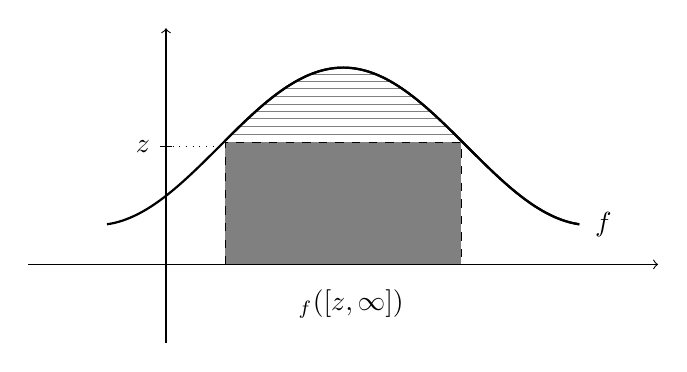
\begin{tikzpicture}
\foreach \i in {0.25,0.6,0.95,1.3,1.65,2.05,2.5,3,3.55} {
\draw[gray] (-0.5+0.3*\i,{1.5+cos deg (-0.5+0.3*\i-1)}) -- (2.5-0.3*\i,{1.5+cos deg (2.5-0.3*\i-1)}) ;};
\fill[gray] (-0.5,0) rectangle (2.5,1.55);
\draw[dashed,thin] (-0.5,0)--(-0.5,1.55)--(2.5,1.55)--(2.5,0);
\draw (-1.17,1.5)--(-1.33,1.5) node[left] {$z$};
\draw (1.1,-0.5) node {$\preim_f([z,\infty])$};
\draw[dotted] (-1.25,1.5)--(-0.5,1.5);
\draw [thick,smooth,samples=100,variable=\x,domain=-2:4] plot (\x,{1.5+cos deg (\x-1)}) node[right=2pt] {$f$};
\draw [thick,smooth,samples=100,variable=\x,domain=-0.5:4] plot (\x,{1.5+cos deg (\x-1)});
\draw[->,thin] (-3,0)--(5,0);
\draw[->,thin] (-1.25,-1)--(-1.25,3);
\end{tikzpicture}}
\end{center}

\v

The following is the pivotal theorem of Lebesgue integration.

\bt[Monotone Convergence Theorem]
Let $(M,\Sigma,\mu)$ be a measure space and let $\{f_n\}_{n\in\N}$ be a sequence of non-negative, measurable
functions $M\to\overline{\R}$ such that $f_{n+1}\geq f_n$ for all $n\in \N$. If there exists a function $f\cl M\to
\overline{\R}$ such that:
\bse
\forall \, m \in M : \ \lim_{n\to\infty}f_n(m) = f(m)
\ese

(i.e.\ $f$ is the pointwise limit of $\{f_n\}_{n\in\N}$), then $f$ is measurable and:
\bse
\lim_{n\to\infty}\int_M\! f_n \, \d \mu = \int_M\! f \, \d \mu
\ese
\et

Observe that this result is in stark contrast with what one may be used from Riemann integration, where pointwise
converge of a sequence of integrable functions $\{f_n\}_{n\in\N}$ is \emph{not} a sufficient condition for the
integral of the limit $f$ to be equal to the limit of the integrals of $f_n$ or, in fact, even for $f$ to be
integrable. For these, we need stronger conditions on the sequence $\{f_n\}_{n\in\N}$, such as uniform converge. \v

The definition of the integral as a supremum is clear and geometrically reasonable. However, it is in general very
difficult to evaluate the integral of any particular function using it. The monotone convergence theorem provides a
much simpler way to evaluate the integral. One can show that, for any non-negative, measurable function $f$, there
exists an increasing sequence $\{s_n\}_{n\in\N}$ of non-negative, measurable, simple functions (which can be
explicitly constructed from $f$) whose pointwise limit is $f$, and hence, we have:
\bse
\int_M\! f \, \d \mu = \lim_{n\to\infty}\int_M\! s_n \, \d \mu
\ese

\v

where the right-hand side can usually be evaluated fairly easily. \v

The monotone convergence theorem can be used to extend some of the properties of integrals of non-negative, measurable
simple functions to non-negative, measurable functions which are not-necessarily simple. \v

We also have the following theorem.

\bt[]
Let $(M,\Sigma,\mu)$ be a measure space, let $f,g\cl M\to \overline{\R}$ be non-negative, measurable functions and
let $c\in [0,\infty)$. Then:
\bse
\displaystyle \int_{M}\! (cf+g) \,\d \mu = c\int_{M}\! f \,\d \mu + \int_{M}\! g \,\d \mu
\ese
\et

Let's prove this!

\bq
Let $\{s_n\}_{n\in\N}$ and $\{t_n\}_{n\in\N}$ be increasing sequences of non-negative, measurable, simple functions
whose pointwise limits are $f$ and $g$, respectively. Then, it is easy to see that $\{cs_n+t_n\}_{n\in\N}$ is an
increasing sequence of non-negative, measurable, simple functions whose pointwise limit is $cf+g$. Hence, by the
monotone converge theorem:
{\setlength{\jot}{10pt}
\begin{align*}
\int_M\! (cf+g) \,\d \mu & = \lim_{n\to\infty}\int_M\! (cs_n+t_n) \, \d \mu\\
& = \lim_{n\to\infty}\biggl(c\int_M\! s_n \, \d \mu+\int_M\! t_n \, \d \mu\biggr)\\
& = c\lim_{n\to\infty}\int_M\! s_n \, \d \mu+\lim_{n\to\infty}\int_M\! t_n \, \d \mu\\
& = c\int_{M}\! f \,\d \mu +\int_{M}\! g \,\d \mu
\end{align*}}
\eq

The previous lemma and the monotone convergence theorem also imply that, for any sequence $\{f_n\}_{n\in\N}$ of
non-negative, measurable functions, we have:
\bse
\int_M \biggl(\sum_{\,n=0}^{\infty}f_n \biggr) \d \mu = \sum_{n=0}^{\infty} \int_M \! f_n \, \d \mu
\ese

Again, note that this result does \emph{not} hold for the Riemann integral unless stronger conditions are places on
the sequence $\{f_n\}_{n\in\N}$. This means that, for the purposes of Lebesgue integration, null sets can be
neglected as they do not change the value of an integral. \v

Finally, we are now in a position to define the full Lebesgue integrable functions (not just for non-negative
functions but for all of them). Since the difference $\infty-\infty$ is not defined, we cannot integrate all
measurable functions. There is, however, a very small extra condition (beyond measurability) that determines the
class of functions to which we can extend our previous definition.

\bd [Lebesgue Integrable Function]
Let $(M,\Sigma,\mu)$ be a measure space and let $f\cl M\to\overline{\R}$. The function $f$ is said to be
\textbf{Lebesgue integrable} if it is measurable and:
\bse
\int_{M}\!|f|\,\d \mu < \infty
\ese
\ed

\bd [$\mathscr{L}^1(M)$]
We denote the set of all integrable functions $M\to\overline{\R}$ by $\mathscr{L}^1_{\R}(M,\Sigma,\mu)$, or simply
$\mathscr{L}^1(M)$.
\ed

For any $f\cl M\to \overline{\R}$, we define $f^+ \coloneqq \max(f,0)$ and $f^- \coloneqq \max(-f,0)$, which are
measurable whenever $f$ is measurable. \v

\bse
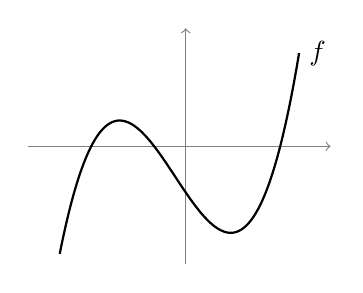
\begin{tikzpicture}[xscale=0.4,yscale=0.5]
\draw[->,thin,gray] (-5,0)--(4.6,0);
\draw[->,thin,gray] (0,-3)--(0,3);
\draw[thick,smooth,samples=100,variable=\x,domain=-4:3.6] plot(\x,{(\x+1)*(\x-3)*(\x+3)*0.13}) node[right] {$f$};
\end{tikzpicture}
\qquad\
\begin{tikzpicture}[xscale=0.4,yscale=0.5]
\draw[->,thin,gray] (-5,0)--(4.6,0);
\draw[->,thin,gray] (0,-3)--(0,3);
\draw[thick,smooth,samples=100,variable=\x,domain=-3:-1] plot(\x,{(\x+1)*(\x-3)*(\x+3)*0.13});
\draw[thick,smooth,samples=100,variable=\x,domain=3:3.6] plot(\x,{(\x+1)*(\x-3)*(\x+3)*0.13}) node[right] {$f^+$};
\draw[thick] (-4,0)--(-3,0);
\draw[thick] (-1,0)--(3,0);
\end{tikzpicture}
\qquad\
\begin{tikzpicture}[xscale=0.5,yscale=0.6]
\draw[->,thin,gray] (-5,0)--(4.6,0);
\draw[->,thin,gray] (0,-3)--(0,3);
\draw[thick,smooth,samples=100,variable=\x,domain=-4:-3] plot(\x,{-(\x+1)*(\x-3)*(\x+3)*0.13});
\draw[thick,smooth,samples=100,variable=\x,domain=-1:3] plot(\x,{-(\x+1)*(\x-3)*(\x+3)*0.13}) node[above=20pt]{$\ f^-$};
\draw[thick] (-3,0)--(-1,0);
\draw[thick] (3,0)--(3.7,0);
\end{tikzpicture}
\ese

\vspace{10pt}

Observe that $f=f^+-f^-$ and $|f|=f^++f^-$. Clearly, we have $f^+\leq|f|$ and $f^-\leq |f|$, and hence:
\bse
\int_{M}\!|f|\,\d \mu < \infty\quad \Leftrightarrow \quad \int_{M}\!f^+\,\d \mu < \infty\ \quad \text{ and } \quad
\int_{M}\!f^-\,\d \mu < \infty
\ese

\bd [Lebesgue Integral]
Let $(M,\Sigma,\mu)$ be a measure space and let $f\cl M\to\overline{\R}$ be integrable. Then, the \textbf{Lebesgue
integral} of $f$ over $M$ with respect to $\mu$ is:
\bse
\int_{M}\!f\,\d \mu \coloneqq \int_{M}\!f^+\,\d \mu -\int_{M}\!f^-\,\d \mu
\ese
\ed

It should be clear that the role of the integrability condition $\int_M |f|\, \d \mu<\infty$ is to prevent the
integral of $f$ from being $\infty-\infty$, which is not defined. \v

The following gives the properties expected of sums and scalar multiples of integrals.

\bt[]
Let $(M,\Sigma,\mu)$ be a measure space, let $f,g \in \mathscr{L}^1(M)$ and let $c \in \R$. Then:
\ben[label=(\roman*)]
\item $|f| \in \mathscr{L}^1(M)$ and $ \displaystyle \biggl| \int_M \! f \, \d \mu \biggr| \leq \int_M \! | f| \, \d
\mu $.
\item $c f \in \mathscr{L}^1(M)$ and $ \displaystyle \int_M \! cf \, \d \mu = c \int_M \! f \, \d \mu$.
\item $f+g \in \mathscr{L}^1(M)$ and $ \displaystyle \int_M \! (f+g) \, \d \mu = \int_M \! f \, \d \mu + \int_M \! g
\, \d \mu$.
\item $\mathscr{L}^1(M)$ is a vector space.
\een
\et

\bt[]
Let $(M,\Sigma,\mu)$ be a measure space and let $f,g \in \mathscr{L}^1(M)$.
\ben[label=(\roman*)]
\item If $f=_{\mathrm{a.e.}}g$, then:
\bse
\displaystyle \int_M\! f \, \d \mu = \int_M\! g \, \d \mu
\ese

\item If $f\leq_{\mathrm{a.e.}}g$, then:
\bse
\displaystyle \int_M\! f \, \d \mu \leq \int_M\! g \, \d \mu
\ese
\een
\et

Just as the monotone convergence theorem was very important for integrals of non-negative, measurable functions,
there is a similar theorem that is important for integrals of functions in $\mathscr{L}^1(X)$.

\bt[Dominated Convergence Theorem]
Let $(M,\Sigma,\mu)$ be a measure space and let $\{f_n\}_{n\in\N}$ be a sequence of measurable functions which
converges almost everywhere to a measurable function $f$. If there exists $g \in \mathscr{L}^1(M)$ such that $|f_n|
\leq_{\mathrm{a.e.}} g$ for all $n \in \N$, then:
\ben[label=(\roman*)]
\item $f \in \mathscr{L}^1(M)$ and $f_n \in \mathscr{L}^1(M)$ for all $n \in \N$.
\item $\displaystyle \lim_{n \to \infty} \int_M \! |f_n-f| \, \d \mu =0$.
\item $\displaystyle \lim_{n \to \infty} \int_M \! f_n \, \d \mu = \int_M \! f \, \d \mu$.
\een
\et

\section{Axiomatic Probability Theory}

In the previous two sections we defined the concept of sample space, and we developed measure theory in a very
abstract and generic way, independently of any probability notion. Now by combining those two notions we can develop
the so called ``axiomatic probability theory''. In other words, axiomatic probability theory can be seen as an
application of the measure theory on the sample space set. \v

Recall from its definition, that the sample space $S$ is just the set of all possible outcomes or results of a random
experiment. By selecting a $\sigma$-algebra (usually denoted by $\mathcal{F}$ in probability theory) on that set, we
can define the measure space $(S, \mathcal{F})$ (usually called Borel space in probability theory). The only
ingredient missing in order to move from the Borel space (i.e.\ measure space) to a measurable space is a specific
choice of measure. $\mu$. \v

Unsurprisingly the measure used in probability theory is called ``probability measure'' or more often in applied
probability theory and statistics ``probability distribution'' and is denoted by $\mu \equiv P$.

\bd[Probability Measure / Distribution]
A \textbf{probability measure} (or probability distribution) $P$ on a Borel space $(S, \mathcal{F})$ is a real-valued
function that maps elements of $\mathcal{F}$ to the real numbers and satisfies the following three axioms:
\ben
\item The probability of an event A is a non-negative real number:
\bse
P(A)\geq 0 \qquad \forall A\in S
\ese

\item The probability that at least one of the events in the entire sample space will occur is 1:
\bse
P(S)=1
\ese

\item Any countable sequence of mutually exclusive events $(A_{1}, A_{2}, \ldots)$ satisfies:
\bse
P\left(\bigcup _{i=1}^{\infty }A_{i}\right)=\sum _{i=1}^{\infty }P(A_{i})
\ese
\een
\ed

This is the formal definition of probability, free of the constraints of naive probability. Finally, given the Borel
space $(S, \mathcal{F})$ and the probability measure $P$ we can define the measure space $(S, \mathcal{F}, P)$ which
we call the ``probability space''.

\bd[Probability Space]
Given a sample space $S$, a $\sigma$-algebra $\mathcal{F}$ and a probability distribution $P$ (that satisfies the
aforementioned three axioms) on the sample space $S$, we define the \textbf{probability space} as the tuple $(S,
\mathcal{F}, P)$.
\ed

A probability space models a real-world process consisting of states that occur randomly. Subsequently, an outcome is
the result of a single execution of the model. Since individual outcomes might be of little practical use, more
complex events are used to characterize groups of outcomes. The collection of all such events is a $\sigma$-algebra
$\mathcal{F}$. Finally, the probability measure $P$ specifies each event's likelihood of happening. \v

Using the definition of probability space and the three axioms we can prove various relation between probabilities of
events.

\bt[]
$P(A^{C}) = 1 - P(A)$
\et

Proving this is quite straight-forward.

\bq
Since the union any event A with its complement $A^C$ gives back the whole sample space, it is:
\begin{align*}
& S = A \cup A^{C} \Rightarrow \\
& P(S) = P(A \cup A^{C}) = P(A) + P(A^{C}) \Rightarrow \\
& P(A^{C}) = P(S) - P(A) \Rightarrow \\
& P(A^{C}) = 1 - P(A)
\end{align*}
\eq

\bt[]
$P(\emptyset) = 0$
\et

Similarly proving this is quite straight-forward.

\bq
Since $S \cup \emptyset = S$ we can set $A = S$ and $A^{C} = \emptyset$ in the previous lemma and we obtain:
\begin{align*}
& P(A^{C}) = 1 - P(A) \Rightarrow \\ & P(\emptyset) = 1 - P(S) = 1 - 1 = 0
\end{align*}
\eq

\bt[]
$P(A \cup B) = P(A) + P(B) - P(A \cap B)$
\et

Another easy proof.

\bq
For any events $A$ and $B$, we have the disjoint union:
\begin{align*}
A \cup B &= (A-B) \cup (A \cap B) \cup (B-A) \Rightarrow \\
P(A \cup B) &= P((A-B) \cup (A \cap B) \cup (B-A)) \\
&= P(A - B) + P(A \cap B) + P(B - A) \\
&= P(A) - P(A \cap B) + P(A \cap B) + P(B)- P(A \cap B) \\
&= P(A) + P(B) - P(A \cap B)
\end{align*}
\eq

\section{Conditional Probability}

\bd[Independent Events]
Two events A and B are called \textbf{independent} if and only if their joint probability equals the product of their
probabilities:
\bse
P(A \cap B) = P(A) P(B)
\ese
\ed

Subsequently, for the union of two independent events by using the lemma we proved previously:
\bse
P(A \cup B) = P(A) + P(B) - P(A) P(B)
\ese

We can now move on, on defining conditional probability.

\bd[Conditional Probability]
Given two events A and B, the \textbf{conditional probability} of A given B is defined as the quotient of the
probability of the joint of events A and B, and the probability of B:
\bse
P(A\mid B)={\frac {P(A\cap B)}{P(B)}}
\ese
\ed

This may be visualized as restricting the sample space to situations in which B occurs.

\vspace{-10pt}

\fig{conditional2}{0.4}

\vspace{-15pt}

Given conditional probability, similarly to independent events we can also define conditionally independent events as
follows.

\bd[Conditionally Independent Events]
Two events A and B are called \textbf{conditionally independent} if and only if, given an event C, their joint
conditional probability equals the product of their conditional probabilities:
\bse
P(A \cap B \mid C) = P(A \mid C) P(B \mid C)
\ese
\ed

Conditional probability is very important in probability theory and its applications since based on the definition we
can prove some very useful theorems that we will be using throughout the notes.

\bt[\textbf{Multiplication Rule}]
\bse
P(B\cap A) = P(A) P(B\mid A)
\ese
\et

\bq
Straight forward by multiplying by $P(B)$ both sides the definition of conditional probability.
\eq

\bt[\textbf{Bayes Rule}]
\bse
P(A\mid B) = \frac{P(B\mid A) P(A)}{P(B)}
\ese
\et

\bq
From multiplication rule by interchanging A with B we get:
\bse
P(A\cap B) = P(B) P(A\mid B)
\ese

But since $P(A\cap B)$ = $P(B\cap A)$ we end up having:
\bse
P(B) P(A\mid B) = P(A) P(B\mid A)
\ese

By solving with respect to $ P(A\mid B)$ we get Bayes rule.
\eq

\bt[\textbf{Law Of Total Probability}]
Given a finite or countably infinite partition of a sample space S, $\{B_{n}:n=1,2,3,\ldots\}$ (in other words, a set
of pairwise disjoint events whose union is the entire sample space) then for any event $A$ of the same probability
space:
\bse
P(A) = \sum_{n} P(A \mid B_{n}) P(B_{n})
\ese
\et

\fig{partition}{0.2}

\bq
From the partition follows:
{\setlength{\jot}{10pt}
\begin{align*}
A &= (A \cap B_{1}) \cup (A \cap B_{2}) \cap \ldots \cap (A \cap B_{n}) \Rightarrow \\
P(A) &= P((A \cap B_{1}) \cup (A \cap B_{2}) \cap \ldots \cap (A \cap B_{n}))\\
&= P(A \cap B_{1}) + P(A \cap B_{2}) + \ldots + P(A \cap B_{n}) \\
&= P(A \mid B_{1}) P(B_{1}) + P(A \mid B_{2}) P(B_{2}) + \ldots + P(A \mid B_{n}) P(B_{n}) \\
&= \sum_{n} P(A \mid B_{n}) P(B_{n})
\end{align*}}
\eq